\documentclass[a4wide, 11pt]{article}
\usepackage{a4, fullpage}
\usepackage[pdftex]{graphicx}
\setlength{\parskip}{0.3cm}
\setlength{\parindent}{0cm}
\setlength{\textheight}{670pt}

\begin{document}

\title{Report - Assignment 3: Artificial Neural Network}

\author{Marcel Ngan \and Thai Tam Nguyen \and Jose Kalladanthyil}

\date{\today}         % inserts today's date

\maketitle            % generates the title from the data above

\section{Introduction}
Artificial neural networks (ANNs) are another way of generalising the target function when it is given a set of input and their corresponding output. One neuron is a linear combination of the attributes, and the weights are transformed by the activation function. A neural network can be more expressive by using a non linear activation function and having multiple layers; it can be more expressive than a linear regression. However, one of the drawbacks of having a more expressive network is that there is a chance of overfitting. We therefore have to find an ANN topology and parameters that express a target function that can classify the unseen data with a small error rate

We tested two types of networks: one with six output neurons classifying each emotion, and a six binary classification network.

\section{Implementation Details}

\subsection{Flow Chart}
\begin{center}
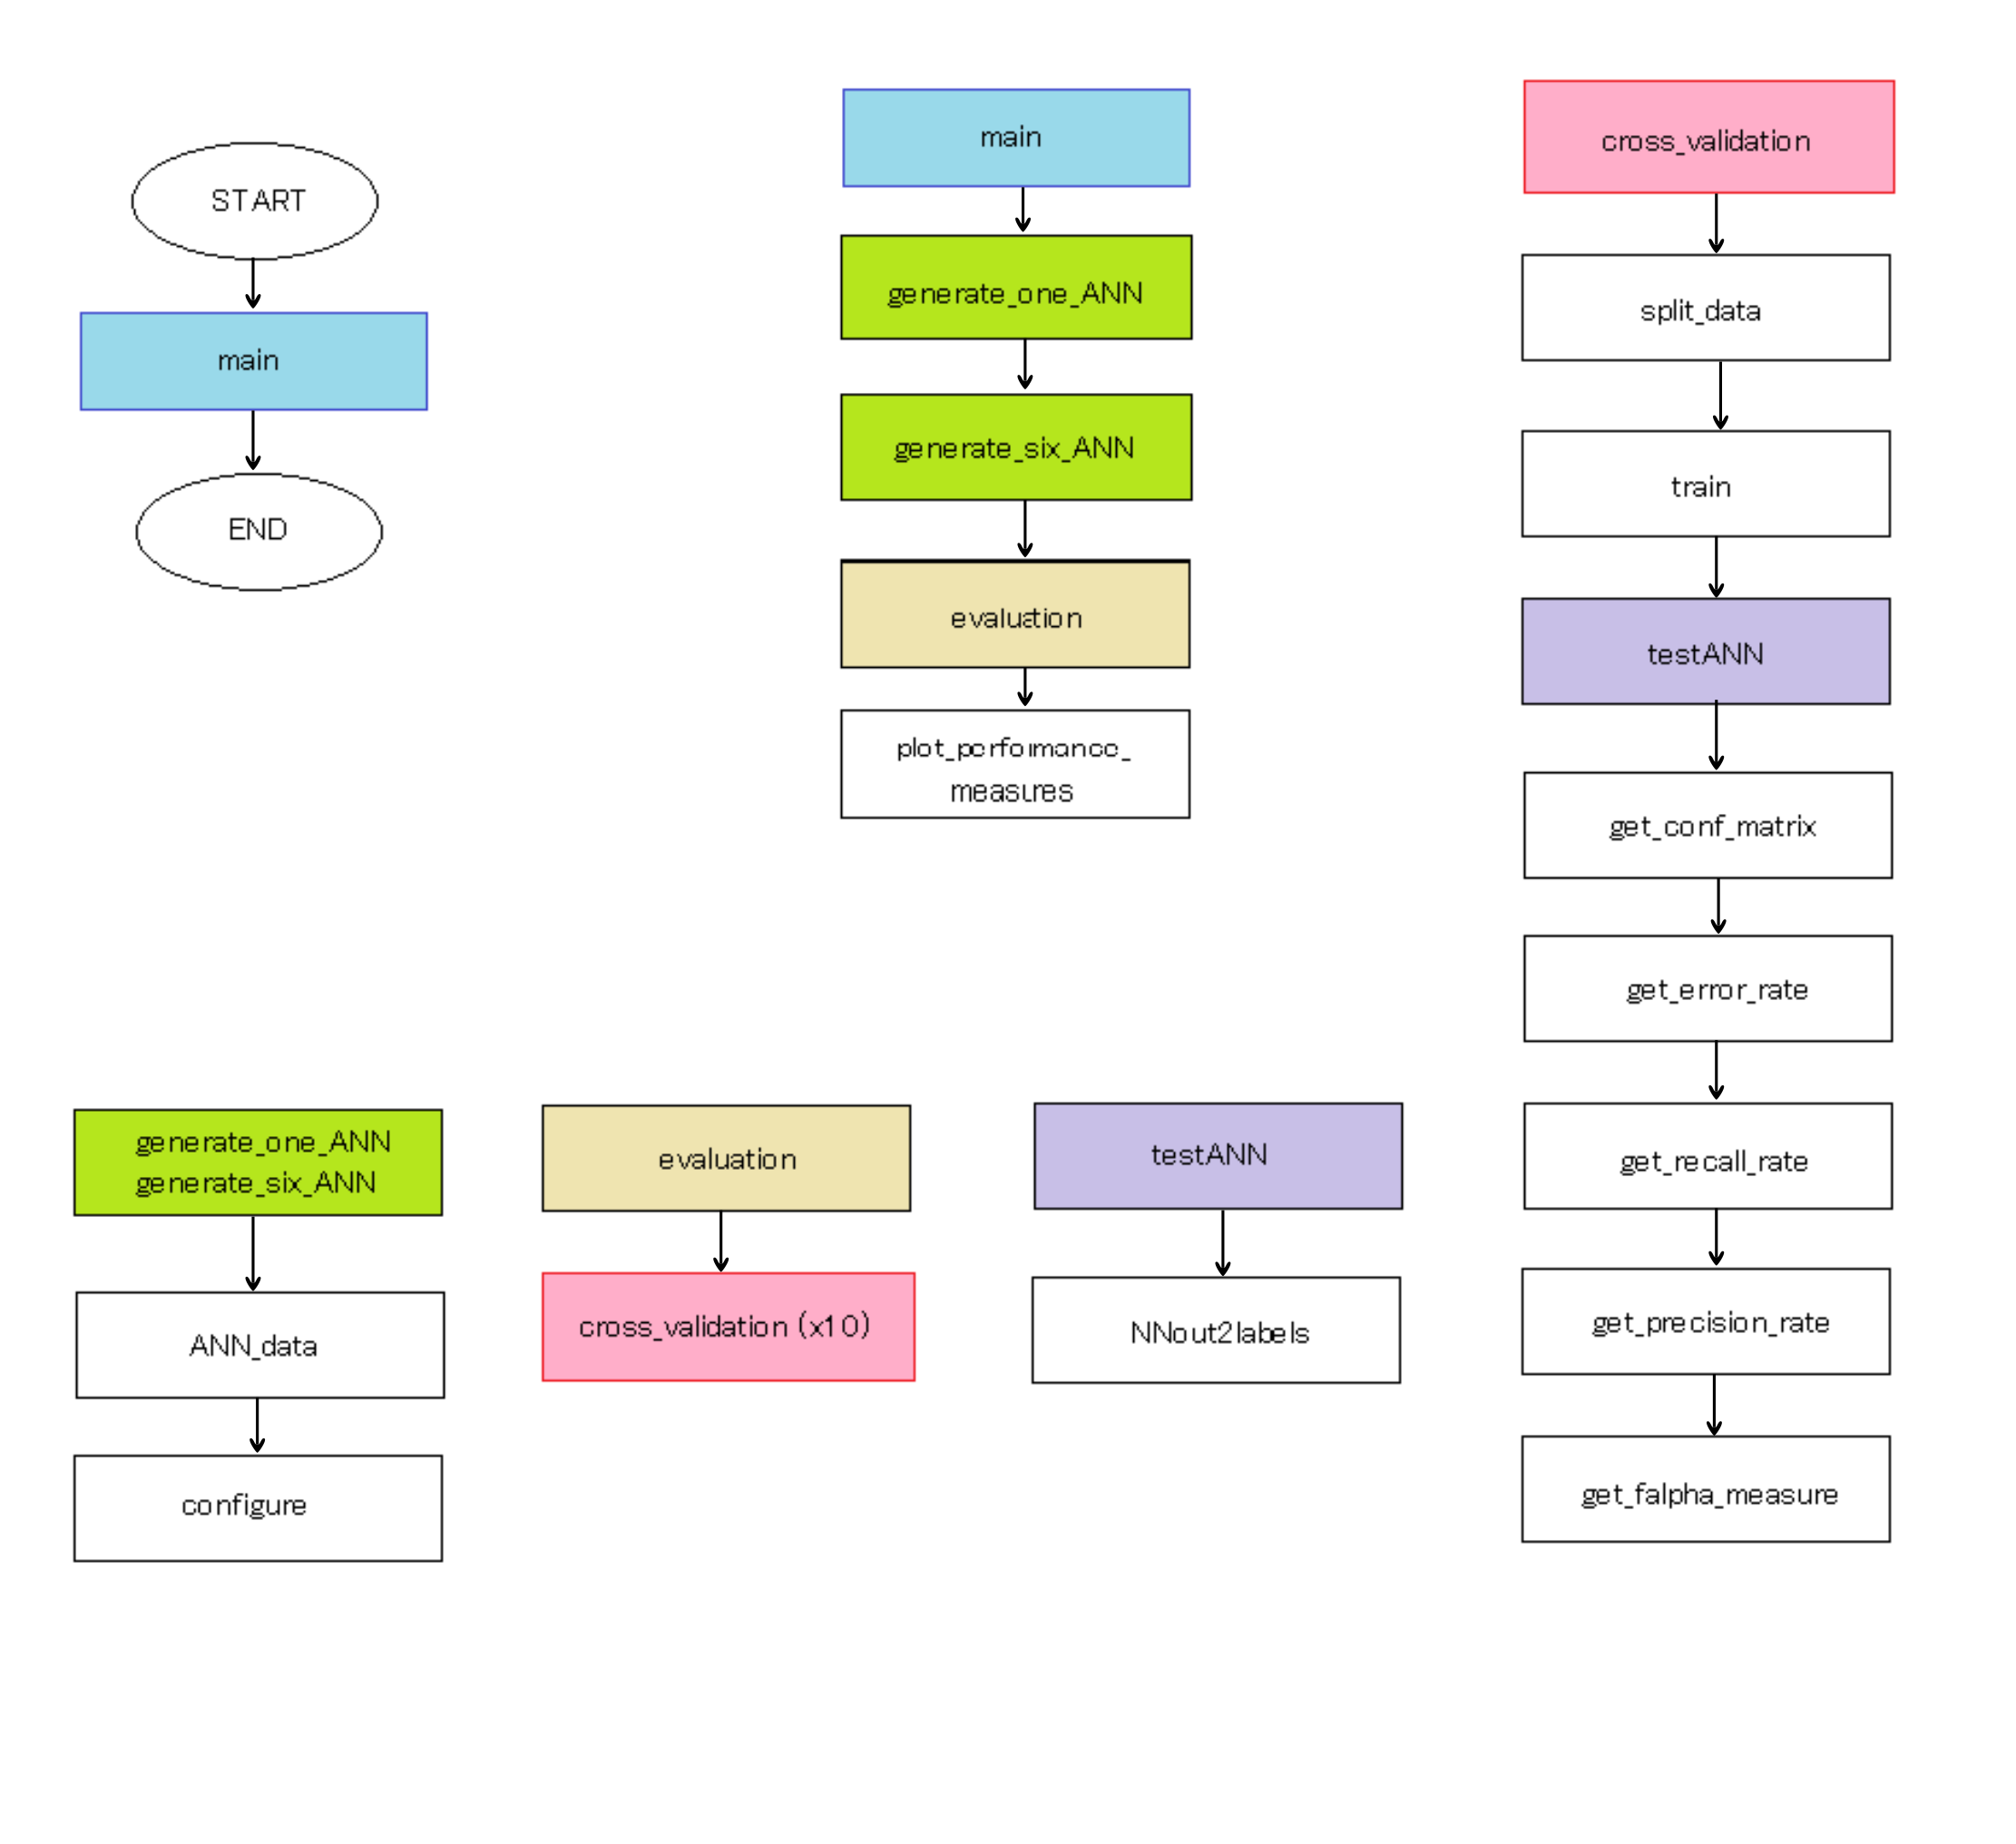
\includegraphics[width=0.5\textwidth]{flowchart.png}
\end{center}

\subsection{Program Flow}
The flowchart above shows the different stages in our program.Our main function calls \textit{generate\_one\_ANN.m} and \textit{generate\_six\_ANN.m}. These in turn create a feed forward neural network and configure them with x2 and y2 from \textit{ANNdata.m}. We create and run our optimised neural network using a different program called \textit{get\_best\_ann}.

\subsection{Main Function}
Our main function \textit{main.m}, it takes in x and y, a matrix of examples and a vector of target values. It generates a configured 6 output neural network and  6 configured single output neural network.  This is followed by \textit{evaluation.m} and \textit{plot\_performance\_measures.m}

The \textit{cross\_validation.m} method is called by our {evaluation.m} 10 times. Its job is to do the one fold of the cross validation where the train set and the validation set are 90\% and 10\% of the 9/10 of the original dataset respectively and the test data is 10\% of the original dataset. After it has trained the network on the thetraining data using one of the training function specified, testANN tests the performance of the networks on the test data. The testANN function combines the 6 binary network into one classifier network. Using the result of the test, we compute the statistics such as confusion matrix, the error rate, and the precision and recall rates for each class, and the F1 measures. After this process is completed for all the 10 folds we calculate the average in the evaluation. The main also plots the average F1 measure for both networks over all 6 classifier against each fold of the cross validation in a bar chart.

\subsection{Optimization}
We have also programmed a separate function \textit{get\_best\_ann.m}, which finds the optimal parameters that we implemented. \textit{get\_best\_ann.m} calls \textit{generate\_ann.m} which creates a cell array of networks, each one with a varying parameters. The \textit{find\_performance.m} splits the data into 10\% validation data and 90\% training data before training each network on the training data. Then it retrieves the performance measure for each network.  We can use these data to determine the optimal parameters.  

\subsection{Cross-validation}
As instructed, we perform 10-fold cross-validation on both types of neural network using the clean data set and, for each type of ANN, produce a confusion matrix, and average values of precision, recall and F1 rates per class.  We also calculate the average classification rate.  We updated \textit{cross\_validation.m} and \textit{evaluation.m} from Assignment 2: Decision Trees Algorithm to be compatible with this assignment.  Similarly to Assignment 2, our \textit{evaluation.m} function takes in all the examples, their corresponding target vector and a neural network as inputs, and performs cross-validation by calling \textit{cross\_validate.m}  10 times.  Each time, our \textit{cross\_validation.m} uses a different fold of data for testing and uses the remaining nine folds for training and validation.  Each time,  \textit{cross\_validation.m} returns a structure containing the predictions, confusion matrix, error rate, precision rates, recall rates and F1 rates.   \textit{evaluation.m} will then store these sets of data in a 1x10 cell array and calculate the final statistics by averaging the individual values.

\subsection{Short Description for all of our functions}
\textit{main.m}: the main function which generate the ANNs and evaluate them.\\
\textit{cross\_validation.m}: does the cross validation for each fold returns all the statistics for the fold such as its confusion matrix, error rate etc\\
\textit{evaluation.m}: does the cross validation for all the datasets and returns the statistics for the whole data such as average error rate etc\\
\textit{generate\_anns.m}: creates a cell array of networks with different paramenters\\
\textit{generate\_one\_ANN.m}: creates a six-output ANN\\
\textit{generate\_six\_ANN.m}: creates six single output ANN.\\
\textit{get\_class\_avg\_palpha\_measure.m}: gets the average F1 measure for that classifier\\
\textit{get\_conf\_matrix.m}: creates the confusion matrix for the fold\\
\textit{get\_error\_rate.m}:  gets the error rate using the target classifier and predicted classifier\\
\textit{get\_falpha\_measure.m}: gets F1 measure rate using recall rate and precision rate\\
\textit{get\_precision\_rate.m}: gets the precision rate for the fold from the classifier and the confusion matrix\\
\textit{get\_recall\_rate.m}: gets the recall rate for the fold from the classifier and the confusion matrix\\
\textit{plot\_performance\_measure.m}: plots a bar graphs showing the performance of the six output ANN and and single output ANNS\\
\textit{split\_data.m}: splits the data set into train data and test data and validation data\\
\textit{testANN.m}: test the trained ANN using the test data\\
\textit{get\_best\_ann.m}: the main function we run to get the optimised parameter\\
\textit{train\_to\_opt.m}: trains the ANN with the given optimisation\\
\textit{find\_performance.m}: finds the best performance of the networks after training\\
\textit{test\_noisy\_data.m}:     takes a noisy data as x and y and a the neural network to test it on\\


\section{Results analysis}
Cross-validation result for one six-outputs network using the clean dataset:

Confusion matrix:
\begin{tabular}{ r r r r r r }
 8.7 & 1.2 & 1 & 0.4 & 1.8 & 0.2 \\
 1.2 & 16.4 & 0.3 & 0.7 & 1.1 & 0.2 \\
 0.3 & 0.6 & 8.4 & 0.0 & 1.0 & 1.7 \\
 0.2 & 0.9 & 0.1 & 19.8 & 0.1 & 0.7 \\
 1.1 & 1.6 & 0.8 & 0.8 & 8.6 & 0.4 \\
 0.2 & 0.4 & 1.2 & 0.2 & 0.3 & 18.7 \\
\end{tabular}

avg\_classification\_rate: 0.7957

avg\_recall\_rates: {[}66.3238 81.9172 70.3897 91.4141 64.6642 88.9630{]}

avg\_precision\_rate: {[}75.9375 77.2475 74.4660 90.2381 67.9223 85.8780{]}

avg\_fold\_falpha\_measure: {[}69.3841 79.2122 69.7254 90.3485 65.7375 86.7083{]}

avg\_class\_falpha\_measure: {[}1x10 double{]}

Cross-validation result for six single-outputs network using the clean dataset:

Confusion matrix:
\begin{tabular}{ r r r r r r }
 9.2 & 1.4 & 0.5 & 0.5 & 1.6 & 0.1 \\
 1.1 & 16.5 & 0.4 & 0.8 & 1.0 & 0.1 \\
 0.6 & 0.5 & 9.5 & 0.3 & 0.2 & 0.9 \\
 0.2 & 0.6 & 0.1 & 20.6 & 0.0 & 0.3 \\
 1.7 & 2 & 0.4 & 0.7 & 8.1 & 0.4 \\
 0.0 & 0.3 & 0.9 & 0.4 & 0.6 & 18.8 \\
\end{tabular}

avg\_classification\_rate: 0.8165

avg\_recall\_rates: {[}69.7682 82.5046 79.4608 94.7828 59.6596 89.4025{]}

avg\_precision\_rate: {[}74.0016 77.0412 81.5694 87.9266 69.6984 91.2713{]}

avg\_fold\_falpha\_measure: {[}70.6262 79.2723 80.0695 91.1224 63.1715 90.2176{]}

avg\_class\_falpha\_measure: {[}1x10 double{]}

The above tables correspond to the confusion matrices produced by each type of ANN on the clean data set.  Generally, the recall and precision rates, and hence F1 measures are quite high, especially for the six single-output networks, to the exception of  sadness, where the average recall rate is lower than in the six-outputs network.  Generally speaking, as seen in the F1 measures that are quite high, both ANNs are quite reliable, with a slight preference towards the six single-output networks. The reliability is reflected in the confusion matrices: the diagonal elements are the highest in the whole matrix, with non-diagonal elements’ values being generally low.

Cross-validation result for one six-outputs network using the noisy dataset:

Confusion matrix:
\begin{tabular}{ r r r r r r }
 1.3 & 1.4 & 1.9 & 1 & 2.3 & 1 \\
 0.5 & 15.1 & 1.3 & 0.7 & 1.1 & 0.2 \\
 0.2 & 0.9 & 12.7 & 1.1 & 1.4 & 2.6 \\
 0.3 & 0.3 & 1.4 & 18.0 & 0.5 & 0.7 \\
 1.0 & 0.8 & 2.0 & 0.6 & 5.3 & 1.3 \\
 0.2 & 0.1 & 1.1 & 1.0 & 1.0 & 18.7 \\
\end{tabular}

 avg\_classification\_rate: 0.7040

avg\_recall\_rates: {[}15.0390 79.4359 66.5952 83.4055 46.7486 84.3165{]}

avg\_precision\_rate: {[}28.7037 82.4255 63.0679 79.7355 48.2348 76.3315{]}

avg\_fold\_falpha\_measure:{[}15.5098 80.1473 64.0028 81.1463 42.6815 79.9249{]}

avg\_class\_falpha\_measure: {[}1x10 double{]}


Cross-validation result for six single-outputs network using the noisy dataset:

Confusion matrix:
\begin{tabular}{ r r r r r r }
 1.6 & 1.5 & 2.7 & 1.2 & 1.5 & 0.4 \\
 0.3 & 16.0 & 1.3 & 0.6 & 0.4 & 0.3 \\
 0.3 & 1.8 & 13.1 & 1.4 & 0.8 & 1.5 \\
 0.3 & 0.7 & 1.2 & 17.8 & 0.3 & 0.9 \\
 1.3 & 1.4 & 2.0 & 0.5 & 5.2 & 0.6 \\
 0.2 & 0.2 & 1.7 & 1.0 & 1.1 & 17.9 \\
\end{tabular}

avg\_classification\_rate: 0.7089

avg\_recall\_rates: {[}18.0304 84.2319 68.5949 84.2376 48.4033 80.8053{]}

avg\_precision\_rate: {[}42.7222 74.2127 59.2551 78.5150 59.5858 83.6882{]}

avg\_fold\_falpha\_measure: {[}23.5225 78.2368 63.4202 80.8765 51.2614 82.0028{]}
   
avg\_class\_falpha\_measure: {[}1x10 double{]}

We can see that our recall and precision rates for both ANNs stay at a very high level, indicating that our ANNs can overcome the problem of noise, regardless of their nature. That is true for all emotions but Anger, whose recall rate drops dramatically from about 69 to about 15.5 in the six-output ANN, and from nearly 70 to about 18, indicating a high amount of false negatives. Both its precision rate and F1 measure are also very low, indicating a high amount of false positives and low reliability respectively. Sadness also has a rather low F1 measure, but stays reasonably high, especially when compared with Sadness. We can conclude that the six single-output networks are quite robust, even when facing noise, while the six-outputs ANN proves more fragile.

\begin{center}
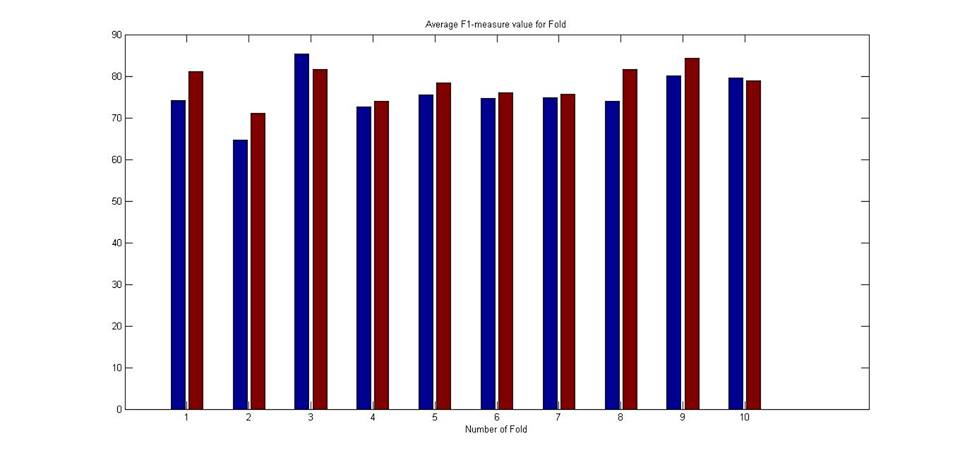
\includegraphics[width=0.5\textwidth]{cleandata.jpg}
\end{center}
Above is the Bar chart of average F1 measures per fold over the 6 classes calculated using the clean dataset.  The blue bar represents the 6-output network and the red bar represents the 6 single-output networks.

\begin{center}
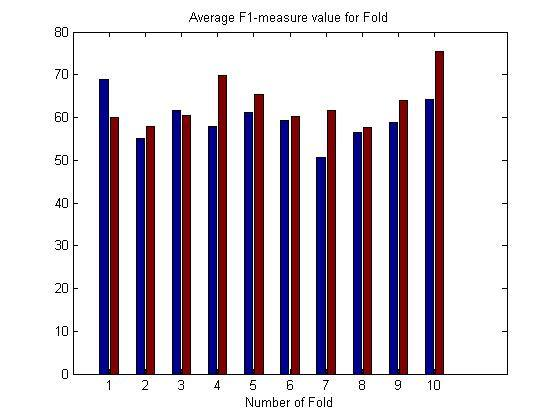
\includegraphics[width=0.5\textwidth]{noisydata.jpg}
\end{center}
Above is the Bar chart of average F1 measures per fold over the 6 classes calculated using the noisy dataset.   The blue bar represents the 6-output network and the red bar represents the 6 single-output networks.

\section{Questions}
\textit{1. Discuss how you obtained the optimal topology and optimal values of network parameters. Describe the performance measure you used (and explain why you preferred it over other measures) and the different topologies / parameters you experimented with.}

At present, we are using values that we have agreed on as optimal values. If we were to optimise our network according to the first fold, or verify our choices using an automated fashion, we would proceed in the following way: modify the number of layers and neurons per layer, change the training and/or activation functions and choose a measure of performance to evaluate the results we get from these changes. This is implemented in get\_best\_ann.m.
We believe that Mean Squared Error (MSE) is a good measure of performance, as it reflects not only the correctness of the classification, but also how close our machine is to actually classifying every element fed to it correctly. However, it does not take into consideration the time taken to compute a result. As such, we think that a quantity defined by MSE/(Average computing time) would be a good indicator of the performance of our ANN.
This would be used to measure the performance of our ANN when changes are brought to the way it functions. For instance, changing the number of layers can lead the machine into overfitting (more on this in question 2). Changing the number of neurons inside each hidden layer can also affect the performance of the system; the more neurons we have, the better is the flexibility of our learning (we can process each data field individually), but the more time it will take to compute a result. We would also measure the changes brought by using different training and activation functions. For example, trainlm, which is known for its efficiency in the machine learning field, or traingd or trainbr for the training functions, and logsig or tansig, which return a 0 or 1 output, for the activation functions. Changing training functions modifies the way the weight of a neuron is updated during the learning process, while changing the activation functions allows us to approximate the target function more or less expressively. Ideally, we want to use a set of functions and ANN topology that minimises our MSE for our validation set, while letting the machine learn (have the training data MSE curve decrease).

\textit{2. Explain what strategy you employed to ensure good generalisation ability of the networks and overcome the problem of overfitting.}

Overfitting in machine learning corresponds to the fact that an ANN does not perform as well on an unknown data set as on its learning set. So if we can avoid overfitting, we can get an ANN that has a relatively good generalisation ability. In order to overcome the problem of overfitting, we manually tested multiple ANN settings. We noticed that the more layers our ANN uses, the faster we encounter a problem of overfitting; while the training error curve steadily decreases, the validation error curve increases, most likely due to overfitting. We therefore chose to use very few layers (ie. 2) as it would force the machine to produce more simple hypotheses, thus keeping overfitting at bay. Matlab can also stop the learning process of our ANN when it has reached the optimal number of epochs. This is useful, because the MSE on the validation set stops decreasing after having reached this optimal number of epochs, while the MSE on the training data keeps on decreasing. If we do not stop the learning process at that point, it may lead to overfitting as the machine will learn, and incorporate, noise into its hypotheses.

\textit{3. Is there any difference in the average classification performance of the two different classification approaches (consider both scenarios, clean and noisy datasets). Discuss the advantages / disadvantages of using 6 single-output NNs vs. 1 six-output NNs.}

Results coming from using the 6 single-output ANNs are slightly better than results given by the six-outputs ANN; the average classification rate is slightly higher for the former (0.71 against 0.70 for noisy data), and so are its F1 measures (particularly visible when using noisy data, emotion Anger). However, in general, there is little difference between using one method or the other. 
In theory, the initial weights of each ANN are set randomly, meaning that, when using the set of 6 single-output ANNs, we are effectively giving each one of them different initial weights. This should affects the training process as they will get updated depending on those initial weightings, regardless of the training function used - the training process for each of the 6 ANNs will differ from one another. This should be a disadvantage when compared to the single six-outputs ANN; even if the weights are randomly assigned, the training process will still lead to a uniform, consistent classifier. But we can see that, in practice, this does not have a strong repercussion on the results we actually get from either ANN. 

\textit{4. In Part VI you optimised the parameters in the first fold only. Ideally, how should the parameters be optimised?}

Optimising the parameters in the first fold only makes these parameters specific to the first fold; if used during cross validation on the all the different folds, these parameters may introduce a bias on the performance, and therefore, on the results given by our ANN. Our measure of performance may not be reliable anymore as our ANN would perform very well if the first fold were used for testing during cross-validation, which would heighten our average classification measures (classification, precision, recall, F1 rates). In opposition, it may perform much worse on completely new data. Ideally, we would like to always test on unseen data. To do this, we reserve one fold of our data set to be used for testing, while the remaining folds are split between training and validation sets. In our case, we would have 1/10th of the data reserved for testing, and 9/10th for the rest. An easy way to split this would be with a 2:1 or 7:2 training:validation ratio. We believe 2:1 to be better as it facilitates calculations in the general case. After having split the data set into these three parts, we want to get the optimal parameters as we train our ANN, and apply them to the test set for each one of the 10 steps of cross-validation. This means we will get 10 sets of optimal parameters, specific to each fold, that have not been pre-computed. By doing this, we can remove the bias introduced by simply using the parameters obtained from analysing the first fold.





\end{document}













